\documentclass[12pt]{scrartcl}

\usepackage[utf8]{inputenc}

\usepackage{mathpazo} % math & rm
% \linespread{1.05}        % Palatino needs more leading (space between lines)
\usepackage[scaled]{helvet} % ss
\usepackage{courier} % tt
\normalfont
\usepackage[T1]{fontenc}

\usepackage{amsthm,amssymb,amsbsy,amsmath,amsfonts,amssymb,amscd}
\usepackage{dsfont}
\usepackage{tasks}
\usepackage{enumitem}
\usepackage[top=2cm, bottom=2cm, left=3cm , right=3cm]{geometry}
\usepackage{tikz}
\usepackage[hidelinks]{hyperref}
\usetikzlibrary{automata,arrows,positioning,calc}

\begin{document}
\begin{center}
	\rule{\textwidth}{1pt}
	\\ \ \\
	{\LARGE \textbf{Lab 1 -- Linear and GP regression}}\\
	\vspace{3mm}
	{\large Short course on Statistical modelling for optimization\\ \vspace{3mm}}
	{\normalsize N. Durrande - J.C. Croix, Universidad Tecnol\'ogica de Pereira, 2017}\\
	\vspace{3mm}
	\rule{\textwidth}{1pt}
	\vspace{5mm}
\end{center}
This lab session is composed of two independent parts: the first one on linear regression and the second one on Gaussian process regression.

\paragraph{}
\noindent One easy way to get a Python distribution with the required packages is to use the Anaconda environment from Continuum Analytics.
A free version of Anaconda can be downloaded and installed from  \url{https://store.continuum.io}. Installing Anaconda will also provide the program ``spyder'' which is a useful scientific python development environment.

\paragraph{}
\noindent
The aim of the four lab sessions will be to study a numerical simulator of a catapult and to find the input settings that give the longest throw. You will need R and the shiny package to be installed on your machine to run the simulator. Once you have them installed, you can run the simulator with the following R commands:
\begin{verbatim}
		library(shiny)
		runGitHub("shinyApps",username="NicolasDurrande",subdir="catapult")
\end{verbatim}
Feel free to take a couple of minutes to play with the simulator to get an understanding of the input influence. In all the labs, we will be interested in the "Breesy" weather conditions.

%%%%%%%%%%%%%%%%%%%%%%%%%%%%%%%%%%%%%%%%%%%%%%%%%
\section{Linear regression}
The aim of this section is to use some data gathered from previous experiments to gather some information on the influence of the various variables and their interactions.

%\subsection*{Data}
\paragraph{Data} The file \emph{lab1\_data.csv} contains the inputs and outputs for 30 experiments. The first 4 columns correspond to the input parameters $x_1$, ..., $x_4$ and the last one gives the distance of the throw.
% \begin{center}
% 	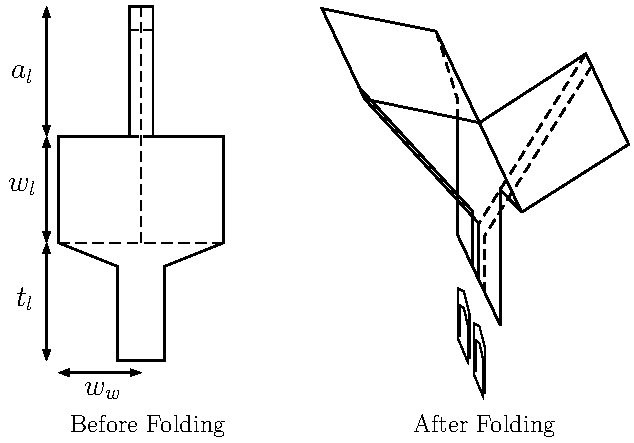
\includegraphics[width=10cm]{figures/helico.pdf}
% \end{center}

% \subsection*{Code}
\paragraph{Code} An incomplete implementation of the lab session is given in the file \emph{lab1\_LR.py}. This sample of code contains the data loading and some elements of a linear regression program.

% \subsection*{Questions}
\paragraph{Q1.} Do some basic data analysis and plotting on $X$ and $F$. Can you identify the variables that have the most influence on the output.

\paragraph{Q2.} Complete the function \texttt{LR} from the file \emph{lab1\_LR.py} such that this function returns the estimate $\hat{\beta}$ and its covariance matrix.

\paragraph{Q3.} Complete the function \texttt{predLR} and build a first regression model based on a constant, a linear effect (say $x_1$) and a quadratic effect for the same variable. Plot the model using the function \texttt{plotModel} and compute the $R^2$. Do some variables seem more influential than others?

\paragraph{Q4.} Repeat the previous question with more than one variable. You may use the function $\texttt{pvalue}$ to test if the effect of some predictors is statistically significant.

\paragraph{Q5.} In the end, what bases functions seem to be appropriate for this function ? Can you find some auxiliary variables (combinations or transformation) of existing variables that are helpful for this problem ?

\paragraph{Q6.} Once you found a model that seems appropriate, validate it by plotting the residuals against the inputs and the outputs.

%%%%%%%%%%%%%%%%%%%%%%%%%%%%%%%%%%%%%%%%%%%%%%%%%
\section{Gaussian process regression}
The code sample \emph{lab1\_GPR.py} will help you for this section. It contains some of the most classical covariance functions (ie kernels). Feel free to add new ones! The demo that was shown this morning is based on the ``shiny'' R package. It can be accessed online here: https://ndurrande.shinyapps.io/GP-explorer.

\paragraph{Q1.} Can you recognize the kernels that are already coded? Give the functions a proper name. Plot various of them and study the influence of the parameters. Why do some of them do not have a length-scale parameter?

\paragraph{Q2.} Complete the function \texttt{sampleGP(x,kern,n,**kwargs)}. This function should return $n$ samples evaluated at $x$ of a centred GP with kernel $kern$. The kernel parameters $\sigma^2$ and $\theta$ may be specified by the user in the input \texttt{**kwargs}.

\paragraph{Q3.} Plot sample paths for various kernels and parameters. What is the influence of the variance and length-scale parameters?

\paragraph{Q4.} Finish writing the function \texttt{predGPR}. It should return the vector of conditional mean $m(x)$ and the conditional covariance matrix $c(x,x)$.

\paragraph{Q5.} Build a model based on a 5 observations of the toy function \texttt{ftest} (input space is $(0,1)$). Plot the model using \texttt{plotModel} and study the influence of the kernel, its parameters and the DoE $X$. Which kernel, parameter values, DoE seem to give the best model? To answer this question, compare the model predictions with actual values of the function on a test set.

\end{document}
